%%%%%%%%%%%%%%%%%%%%%%%%%%%%%%%%%%%%%%%%
% datoteka diploma.tex
%
% vzorčna datoteka za pisanje diplomskega dela v formatu LaTeX
% na UL Fakulteti za matematiko in fiziko
%
% vkup spravil Gašper Fijavž, december 2010
% množica popravkov v januarju, februarju marcu 2011
% verzijo 29. marec 2011 za FMF 19.9.2013 prilagodil Rok Mihevc
%%%%%%%%%%%%%%%%%%%%%%%%%%%%%%%%%%%%%%%%

\documentclass[a4paper, oneside, 12pt]{book}

\usepackage[utf8]{inputenc}   % omogoča uporabo slovenskih črk kodiranih v formatu UTF-8 
\usepackage[slovene,english]{babel}    % naloži, med drugim, slovenske delilne vzorce
\usepackage[pdftex]{graphicx}  % omogoča vlaganje slik različnih formatov 
\usepackage{fancyhdr}          % poskrbi, na primer, za glave strani
\usepackage{amssymb}           % dodatni simboli
\usepackage{amsmath}           % eqref, npr.
\usepackage{verbatim}           % \begin{comment} in \end{comment}
\usepackage{float}
\usepackage{tikz}

\renewcommand{\baselinestretch}{1.3} % ustrezen razmik med vrsticami

%oznake strani

\renewcommand{\chaptermark}[1]%
{\markboth{\MakeUppercase{\thechapter.\ #1}}{}} \renewcommand{\sectionmark}[1]%
{\markright{\MakeUppercase{\thesection.\ #1}}} \renewcommand{\headrulewidth}{0.5pt} \renewcommand{\footrulewidth}{0pt} 
\fancyhf{}
\fancyhead[LE,RO]{\sl \thepage} \fancyhead[LO]{\sl \rightmark} \fancyhead[RE]{\sl \leftmark}

\newcommand{\BibTeX}{{\sc Bib}\TeX}

\newcommand{\autfont}{\Large}
\newcommand{\titfont}{\LARGE\bf}
\newcommand{\clearemptydoublepage}{\newpage{\pagestyle{empty}\cleardoublepage}}
\setcounter{tocdepth}{1}	      % globina kazala

% konstrukti
\newtheorem{izrek}{Izrek}[chapter]
\newtheorem{trditev}{Trditev}[izrek]
\newenvironment{dokaz}{\emph{Dokaz.}\ }{\hspace{\fill}{$\Box$}}

\begin{document}
\selectlanguage{slovene}
\frontmatter
\setcounter{page}{1} %
\renewcommand{\thepage}{}       % preprecimo težave s številkami strani v kazalu 

\begin{comment}

%naslovnica
\thispagestyle{empty}%
\begin{center}
  {\large\sc Univerza v Ljubljani\\%
    Fakulteta za Matematiko in Fiziko\\%
    Oddelek za Fiziko\\%
  Univerzitetni študij, naravoslovna smer}%
  \vskip 10em%
  {\autfont Rok Mihevc \par}%
  {\titfont Kraške vrtače Dinarskega krasa \par}%
  {\vskip 2em \textsc{DIPLOMSKO DELO}\par}%
  \vfill\null%
  {\large \textsc{Mentor}: prof.\ dr.  Rudolf Podgornik\par}%
%  {\large \textsc{Somentor}:  izr.\ prof.\ dr. \par}%
  {\vskip 2em \large Ljubljana, 2013 \par}%
\end{center}
% prazna stran
\clearemptydoublepage


% prazna stran
\clearemptydoublepage

%%%%%%%%%%%%%%%%%%%%%%%%%%%%%%%%%%%%%%%%
% izjava o avtorstvu
\vspace*{1cm}
\begin{center} 
  {\Large \textbf{\sc Izjava o avtorstvu diplomskega dela}}
\end{center}

\vspace{1cm}
\noindent Spodaj podpisani Rok Mihevc,
z vpisno številko \textbf{28030017}, sem avtor  diplomskega dela z naslovom: Kraške vrtače Dinarskega krasa

\vspace{0.5cm}
\emph{Vzorec diplomskega dela}

\vspace{1.5cm}
\noindent S svojim podpisom zagotavljam, da:
\begin{itemize}
  \item sem diplomsko delo izdelal samostojno pod mentorstvom 
    prof.\ dr.\ \mbox{Rudolfa} \mbox{Podgornika}, %in somentorstvom izr.\ prof.\ dr.\,

  \item	so elektronska oblika diplomskega dela, naslov (slov., angl.), povzetek (slov., angl.) ter ključne besede (slov., angl.) identični s tiskano obliko diplomskega dela
\end{itemize}

\vspace{1cm}
\noindent V Ljubljani, dne 11. januarja 2013 \hfill Podpis avtorja:

% prazna stran
\clearemptydoublepage

%%%%%%%%%%%%%%%%%%%%%%%%%%%%%%%%%%%%%%%%
% zahvala
\thispagestyle{empty}\mbox{}\vfill\null\it%
Na tem mestu zapišite, komu se zahvaljujete za izdelavo diplomske naloge. Pazite, da ne boste koga pozabili. Utegnil vam bo zameriti. Temu se da izogniti tako, da pozabite na celo zahvalo.
\rm\normalfont

% prazna stran
\clearemptydoublepage

%%%%%%%%%%%%%%%%%%%%%%%%%%%%%%%%%%%%%%%%
% posvetilo
\thispagestyle{empty}\mbox{}{\vskip0.20\textheight}\mbox{}\hfill\begin{minipage}{0.55\textwidth}%
  Svoji dragi Alenčici.
  \normalfont\end{minipage}

% prazna stran
\clearemptydoublepage

%%%%%%%%%%%%%%%%%%%%%%%%%%%%%%%%%%%%%%%%
% ODREZANA NASLOVNICA ITD. DO KAZALA
\end{comment}
%%%%%%%%%%%%%%%%%%%%%%%%%%%%%%%%%%%%%%%%

%%%%%%%%%%%%%%%%%%%%%%%%%%%%%%%%%%%%%%%%
% kazalo
\def\thepage{}% preprecimo tezave s stevilkami strani v kazalu 
\tableofcontents{}

%%%%%%%%%%%%%%%%%%%%%%%%%%%%%%%%%%%%%%%%
% ODREZAN POVZETEK  ITD.
\begin{comment}
%%%%%%%%%%%%%%%%%%%%%%%%%%%%%%%%%%%%%%%%

% prazna stran
\clearemptydoublepage

%%%%%%%%%%%%%%%%%%%%%%%%%%%%%%%%%%%%%%%%
% povzetek 
\addcontentsline{toc}{chapter}{Povzetek}
\chapter*{Povzetek}
V vzorcu je predstavljen postopek priprave diplomskega dela z uporabo okolja \LaTeX. Vaš povzetek mora sicer vsebovati približno 100 besed, ta tukaj je odločno prekratek.
% prazna stran
\clearemptydoublepage

%%%%%%%%%%%%%%%%%%%%%%%%%%%%%%%%%%%%%%%%
% abstract
\selectlanguage{english}
\addcontentsline{toc}{chapter}{Abstract}
\chapter*{Abstract}
This sample document presents an approach to typesetting your BSc thesis using \LaTeX. A proper abstract should contain around 100 words which makes this one way too short.
\selectlanguage{slovene}
% prazna stran
\clearemptydoublepage

%%%%%%%%%%%%%%%%%%%%%%%%%%%%%%%%%%%%%%%%
% ODREZAN POVZETEK  ITD.
\end{comment}
%%%%%%%%%%%%%%%%%%%%%%%%%%%%%%%%%%%%%%%%

%%%%%%%%%%%%%%%%%%%%%%%%%%%%%%%%%%%%%%%%
\mainmatter
\setcounter{page}{1}
\pagestyle{fancy}

\chapter{Uvod}
\label{ch1}
Namen tega dela je na podlagi digitalnega modela reliefa dokumentirati in statistično preučiti velik vzorec realnih kraških vrtač na slovenskem Dinarskem krasu, predlagati analitično funkcijo, ki bi opisala idealno vrtačo, ter na podlagi le-te poiskusiti modelirati naravne procese, ki povzročajo nastanek in obliko vrtač.

Vrtače so zaobljene lijakaste globeli, globine nekaj metrov in premera nekaj deset metrov. Obstaja več geomorfoloških modelov njihovega nastanka.

\begin{figure}[H]
  \begin{center}
    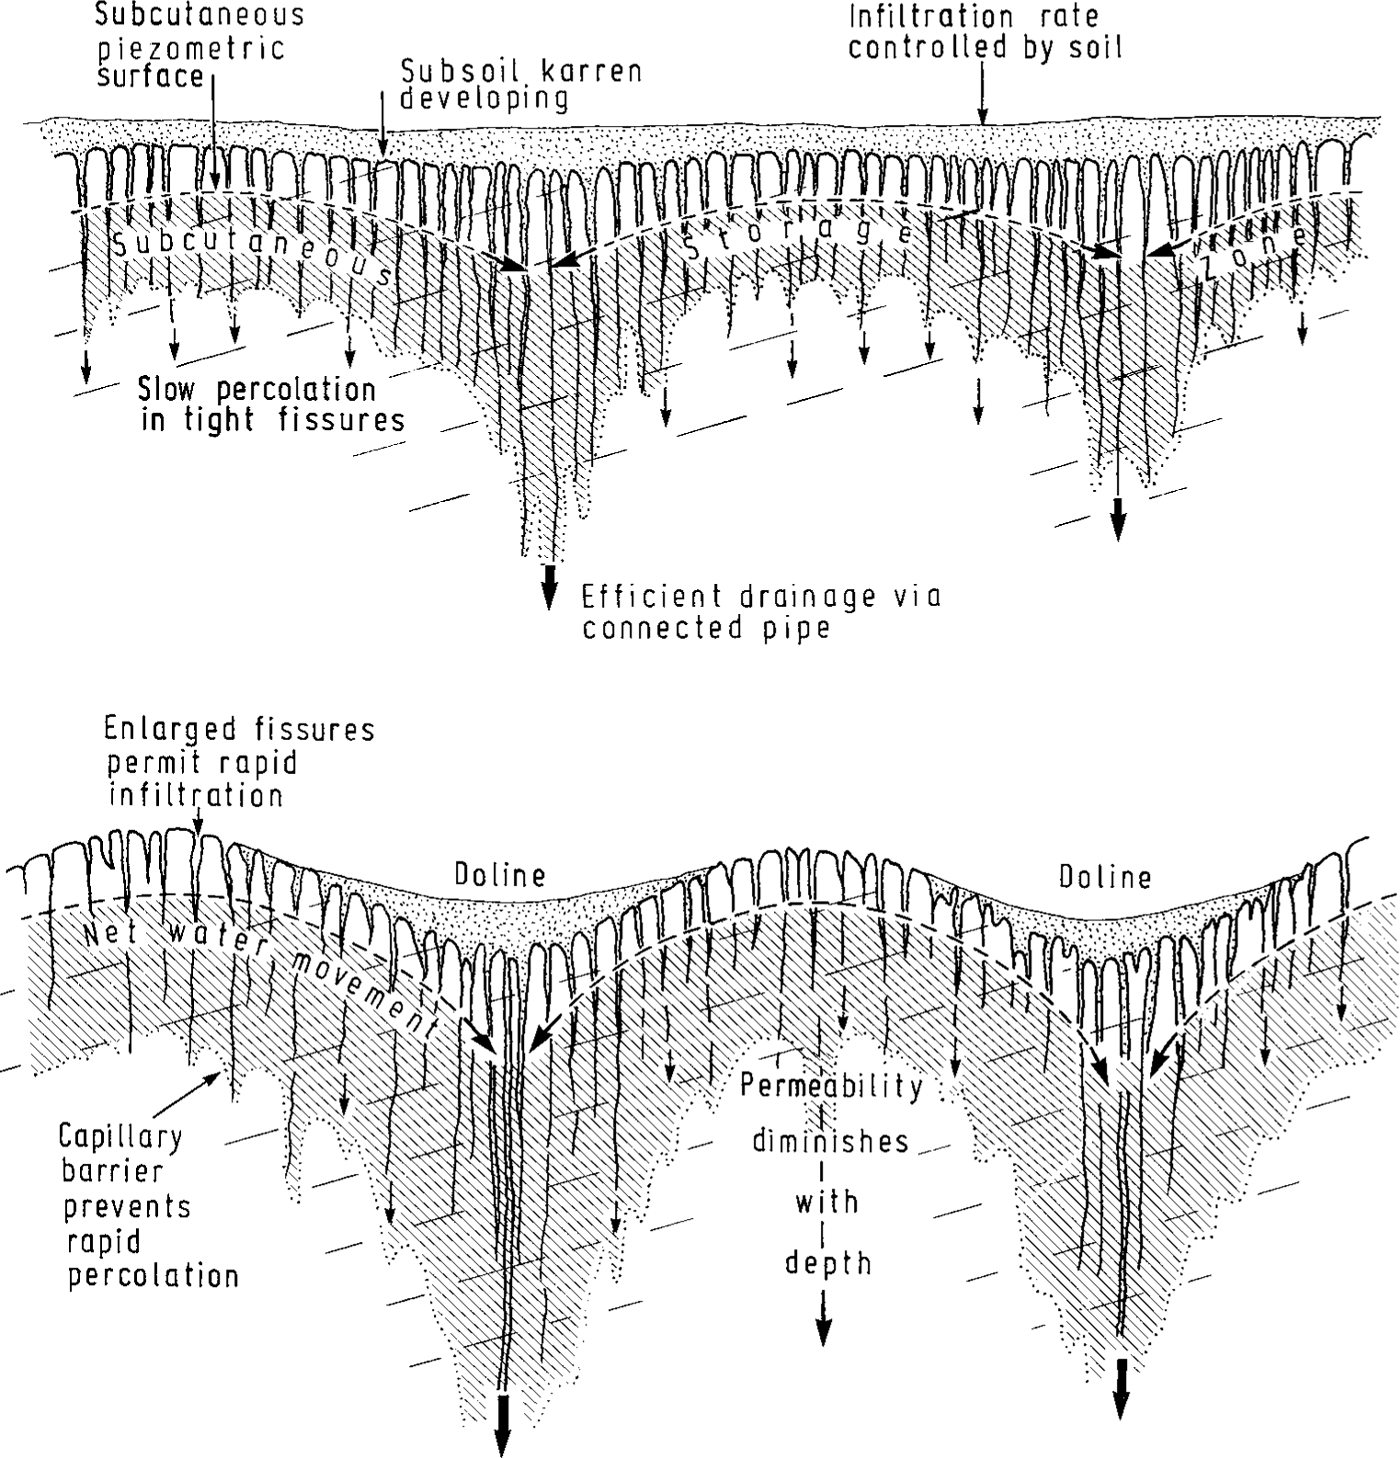
\includegraphics[width=13cm]{slike/vrtaca-ford-williams}
  \end{center}
  \caption{Priljubljena geomorfološka shema za razlago vrtač. Vir: \cite{ford2007karst}}
  \label{fig:vrtaca-ford-williams}
\end{figure}

Za študij realnih vrtač uporabimo digitalni model reliefa Menišije (Slika \ref{fig:menisija-karta}) ločljivosti 1m, ki omogoča zanesljivo identifikacijo in študij vrtačter udornic (Slika \ref{fig:menisija-relief}).

\begin{figure}[H]
  \centering
  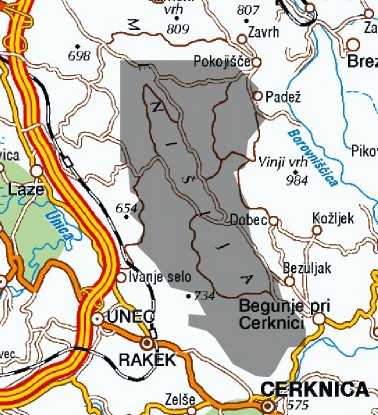
\includegraphics[width=8cm]{slike/menisija-karta}
  \caption{Menišija, $60 km^2$ veliko območje med Cerknico in Logatcem vsebuje nekaj tisoč vrtač in več udornic in predstavlja približno odstotek slovenskega krasa. Vir: Geopedia, Geodetski inštitut Slovenije}
  \label{fig:menisija-karta}
\end{figure}

Površje Menišije sestavljajo plasti krednega apnenca (starost nastanka 135-65 miljonov let), ki so na površje prišli zaradi odgodkov povezanih s podrivanjem Adriatske plošče (17-7 miljonov let). Menišija je bila uravnano kraško polje do 3.5 miljona let pred sedanjostjo, ko se je zaradi tektonske aktivnosti dvignila nad okolico in so bili vzpostavljeni hidrološki pogoji za nastanek vrtač. Hitrost zniževanja (denudacije) kraškega površja se ocenjuje na 20-50 m / miljon let, torej se je površje Menišije v času od nastanka znižalo za 70-175m, hkrati pa so se v njem pojavile vrtače, udornice in brezstrope jame. (Citati: Vrabec, Ford-Williams, Gams)

\begin{figure}[H]
  \begin{center}
    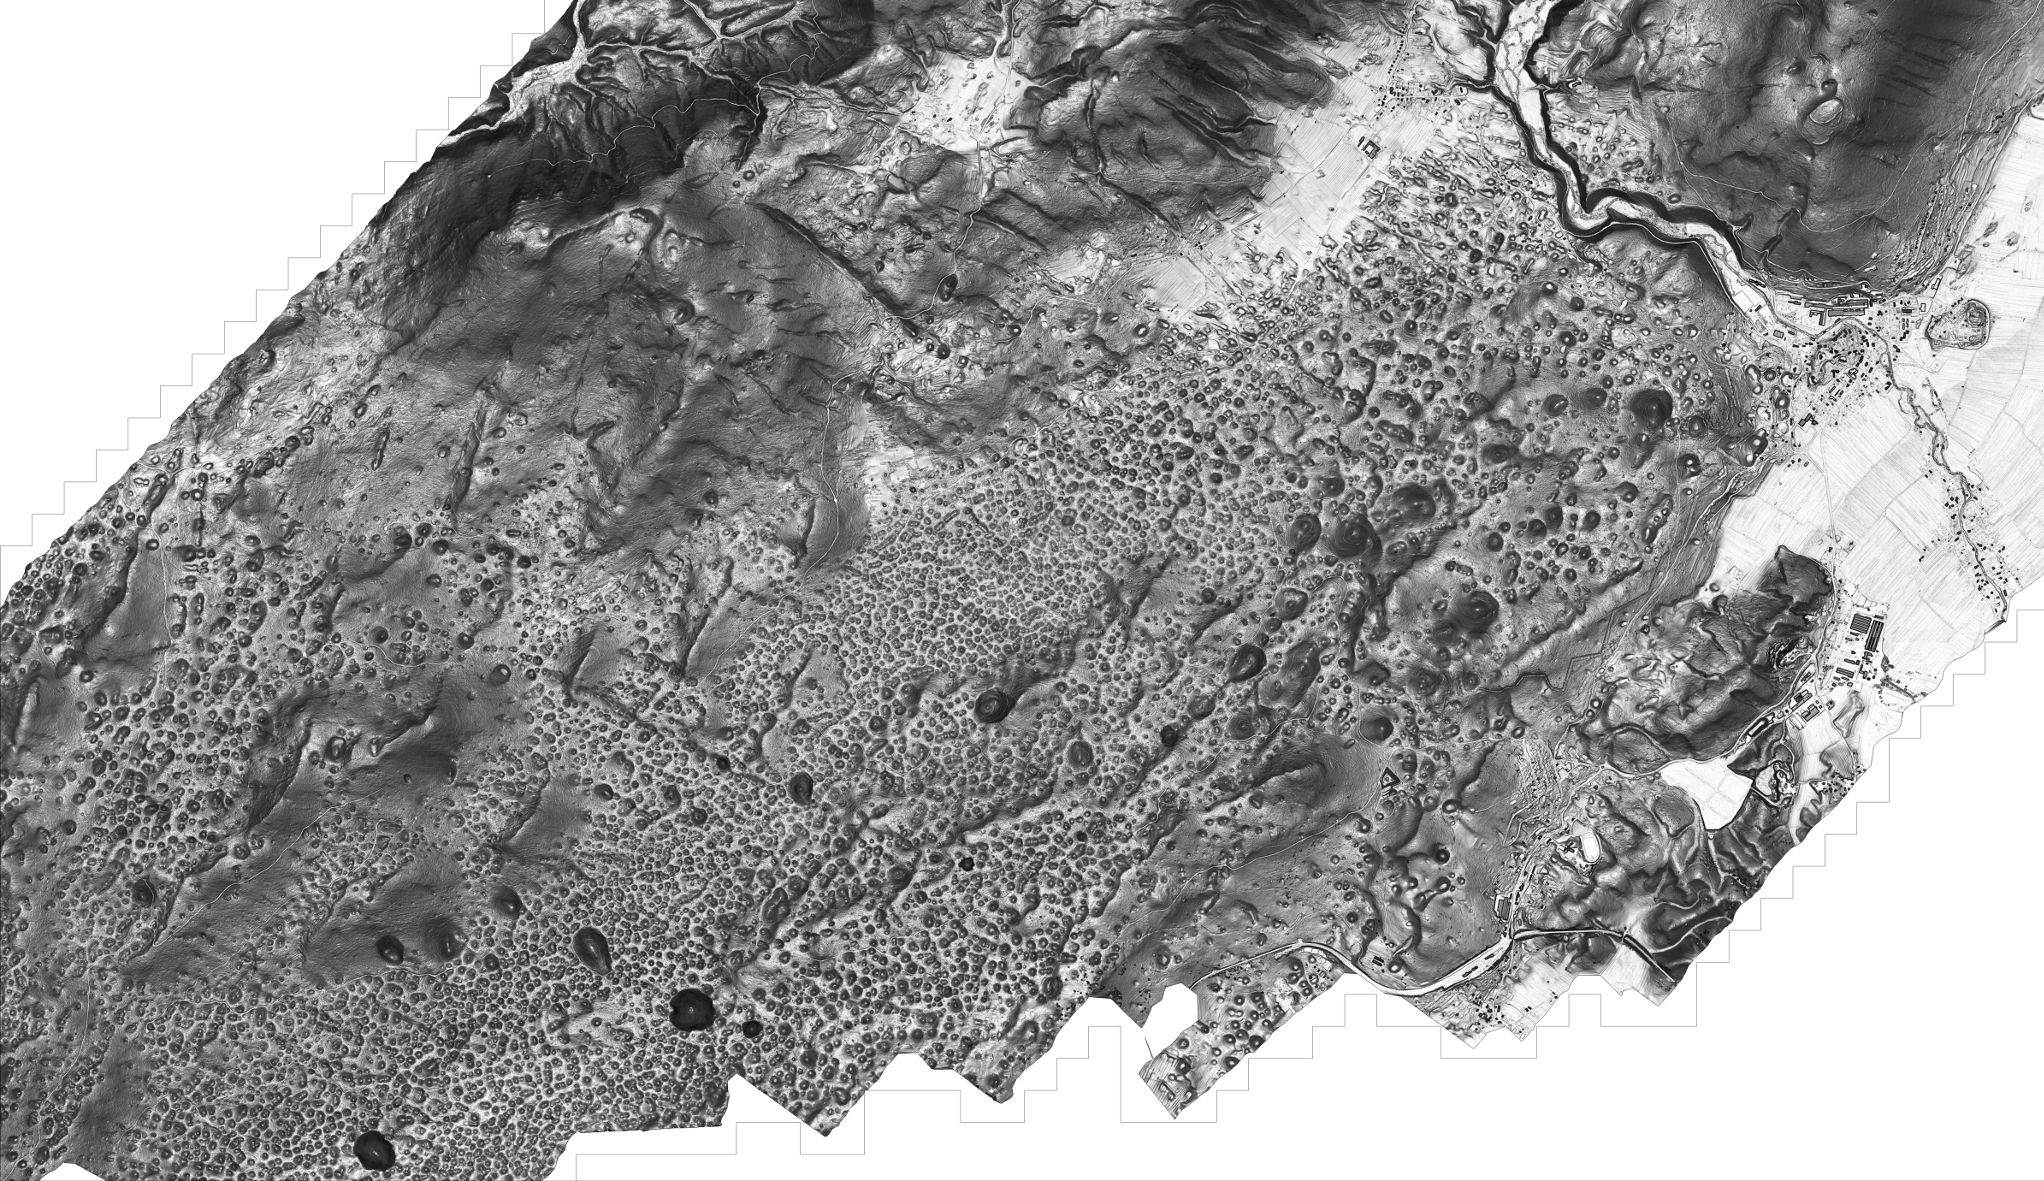
\includegraphics[width=12cm]{slike/menisija-relief}
  \end{center}
  \caption{Senčen 3D relief dela Menišije uporabljen v tej nalogi. Vir: Geodetski inštitur Slovenije \cite{LAK} po metodi \cite{Kobler20079}.}
  \label{fig:menisija-relief}
\end{figure}
\chapter{Preučevanje realnih vrtač}
\label{realne-vrtace}
Identifikacijo velike količine se lotimo s segmentacijo po konkavnosti, kot predlaga \cite{doctor13}. Točke, ki so nižje od svoje okolice imajo nižji indeks konkavnosti, točke višje od svoje okolice pa višjega. Pri tem je pomembna tudi pametna izbiro okolice - od nje je odvisno kako velike konkavnosti bomo zaznali. Končno zavržemo konveksne dele površja in konkavne odberemo izberemo kot vrtače. Rezultat vidimo na sliki \ref{fig:menisija-vrtace}. Opaziti velja, da izbrana metoda segmetacije del robov konkavnih objektov klasificira kot konkavne in zato podceni radij. Za naše namene to ni pretirano moteče, saj to podcenitev zlahka kompenziramo kasneje.

\begin{figure}[H]
  \begin{center}
    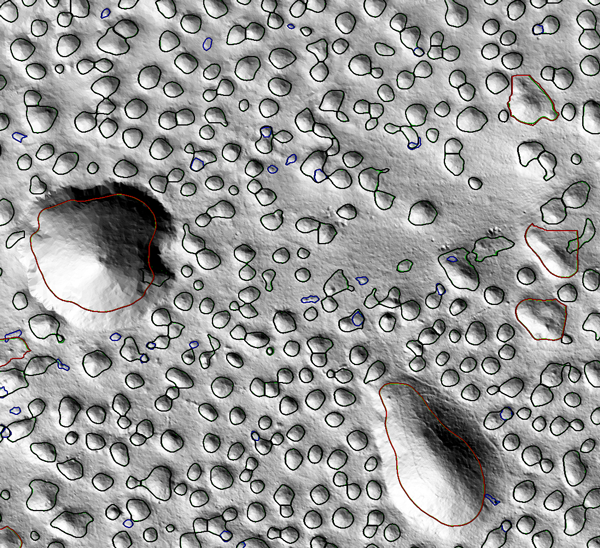
\includegraphics[width=13cm]{slike/menisija-vrtace}
  \end{center}
  \caption{Del od 8687 zaznanih konkavnih objektov na območju Menišije. Poleg vrtač, so na sliki vidne tudi udornice.}
  \label{fig:menisija-vrtace}
\end{figure}


Najdeni konkavni objekti imajo porazdelitev efektivnih polmerov (\mbox{$r_{eff}=\frac{\sqrt{A_{eff}}}{\pi}$}), kot vidno na sliki \ref{fig:menisija-polmeri-hist}.

\begin{figure}[H]
  \centering
  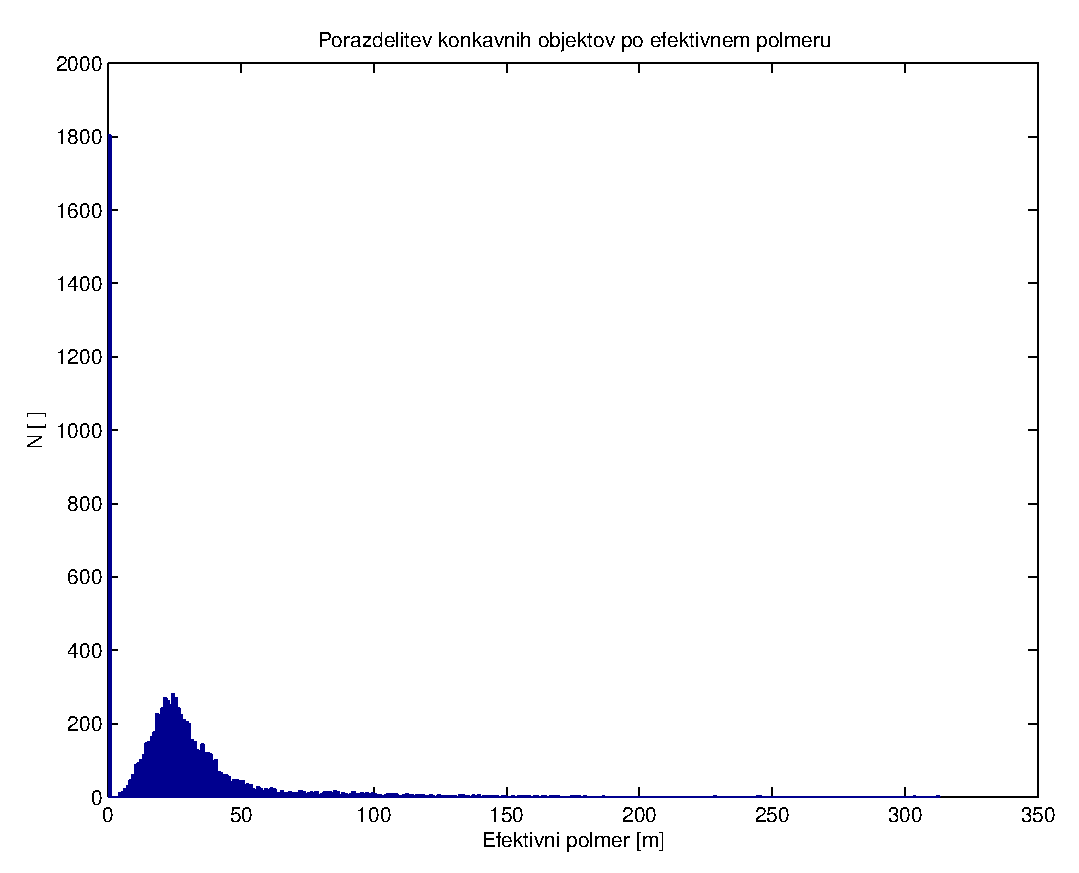
\includegraphics{slike/menisija-polmeri-hist}
  \caption{Polmeri konkavnih objektov v Menišiji, vrh pade v razred od 16m do 17m}
  \label{fig:menisija-polmeri-hist}
\end{figure}

To daje slutiti, da obstaja ravnovesna velikost vrtače, h kateri konvergirajo vse konkavne oblike v območju ne glede na njihov nastanek.
To nas napelje na misel, da obstaja tudi ravnovesna oblika vrtače, ki bi se pojavila na idelani podlagi, če bi preteklo dovolj časa.

Posamezne realne vrtače zaradi lokalnih pogojev in zgodovine razvoja reliefa niso simetrične, a zdi se da so si med seboj podobne. Da bi ugotovili idealno obliko vrtače izračunamo povprečje velikega števila realnih vrtač. Uporabimo dva pristopa - pri prvem (Slika \ref{fig:menisija-vrtaca}) vrtače različnih velikosti raztegnemo, pri drugem (Slika \ref{fig:menisija-vrtace-po-razredih}) pa jih razdelimo v velikostne razrede in jih povprečimo znotraj le-teh. 

\begin{figure}[H]
  \centering
  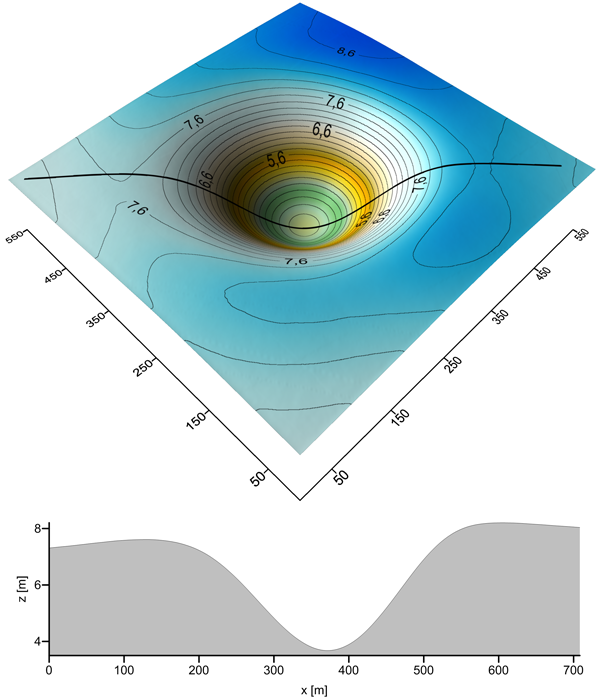
\includegraphics[width=13cm]{slike/menisija-vrtaca}
  \caption{Povprečje 8687 realnih vrtač z območja Menišije, pred povprečjem so bile vrtače raztegnjene na velikost največje v setu.}
  \label{fig:menisija-vrtaca}
\end{figure}

\begin{figure}
  \centering
  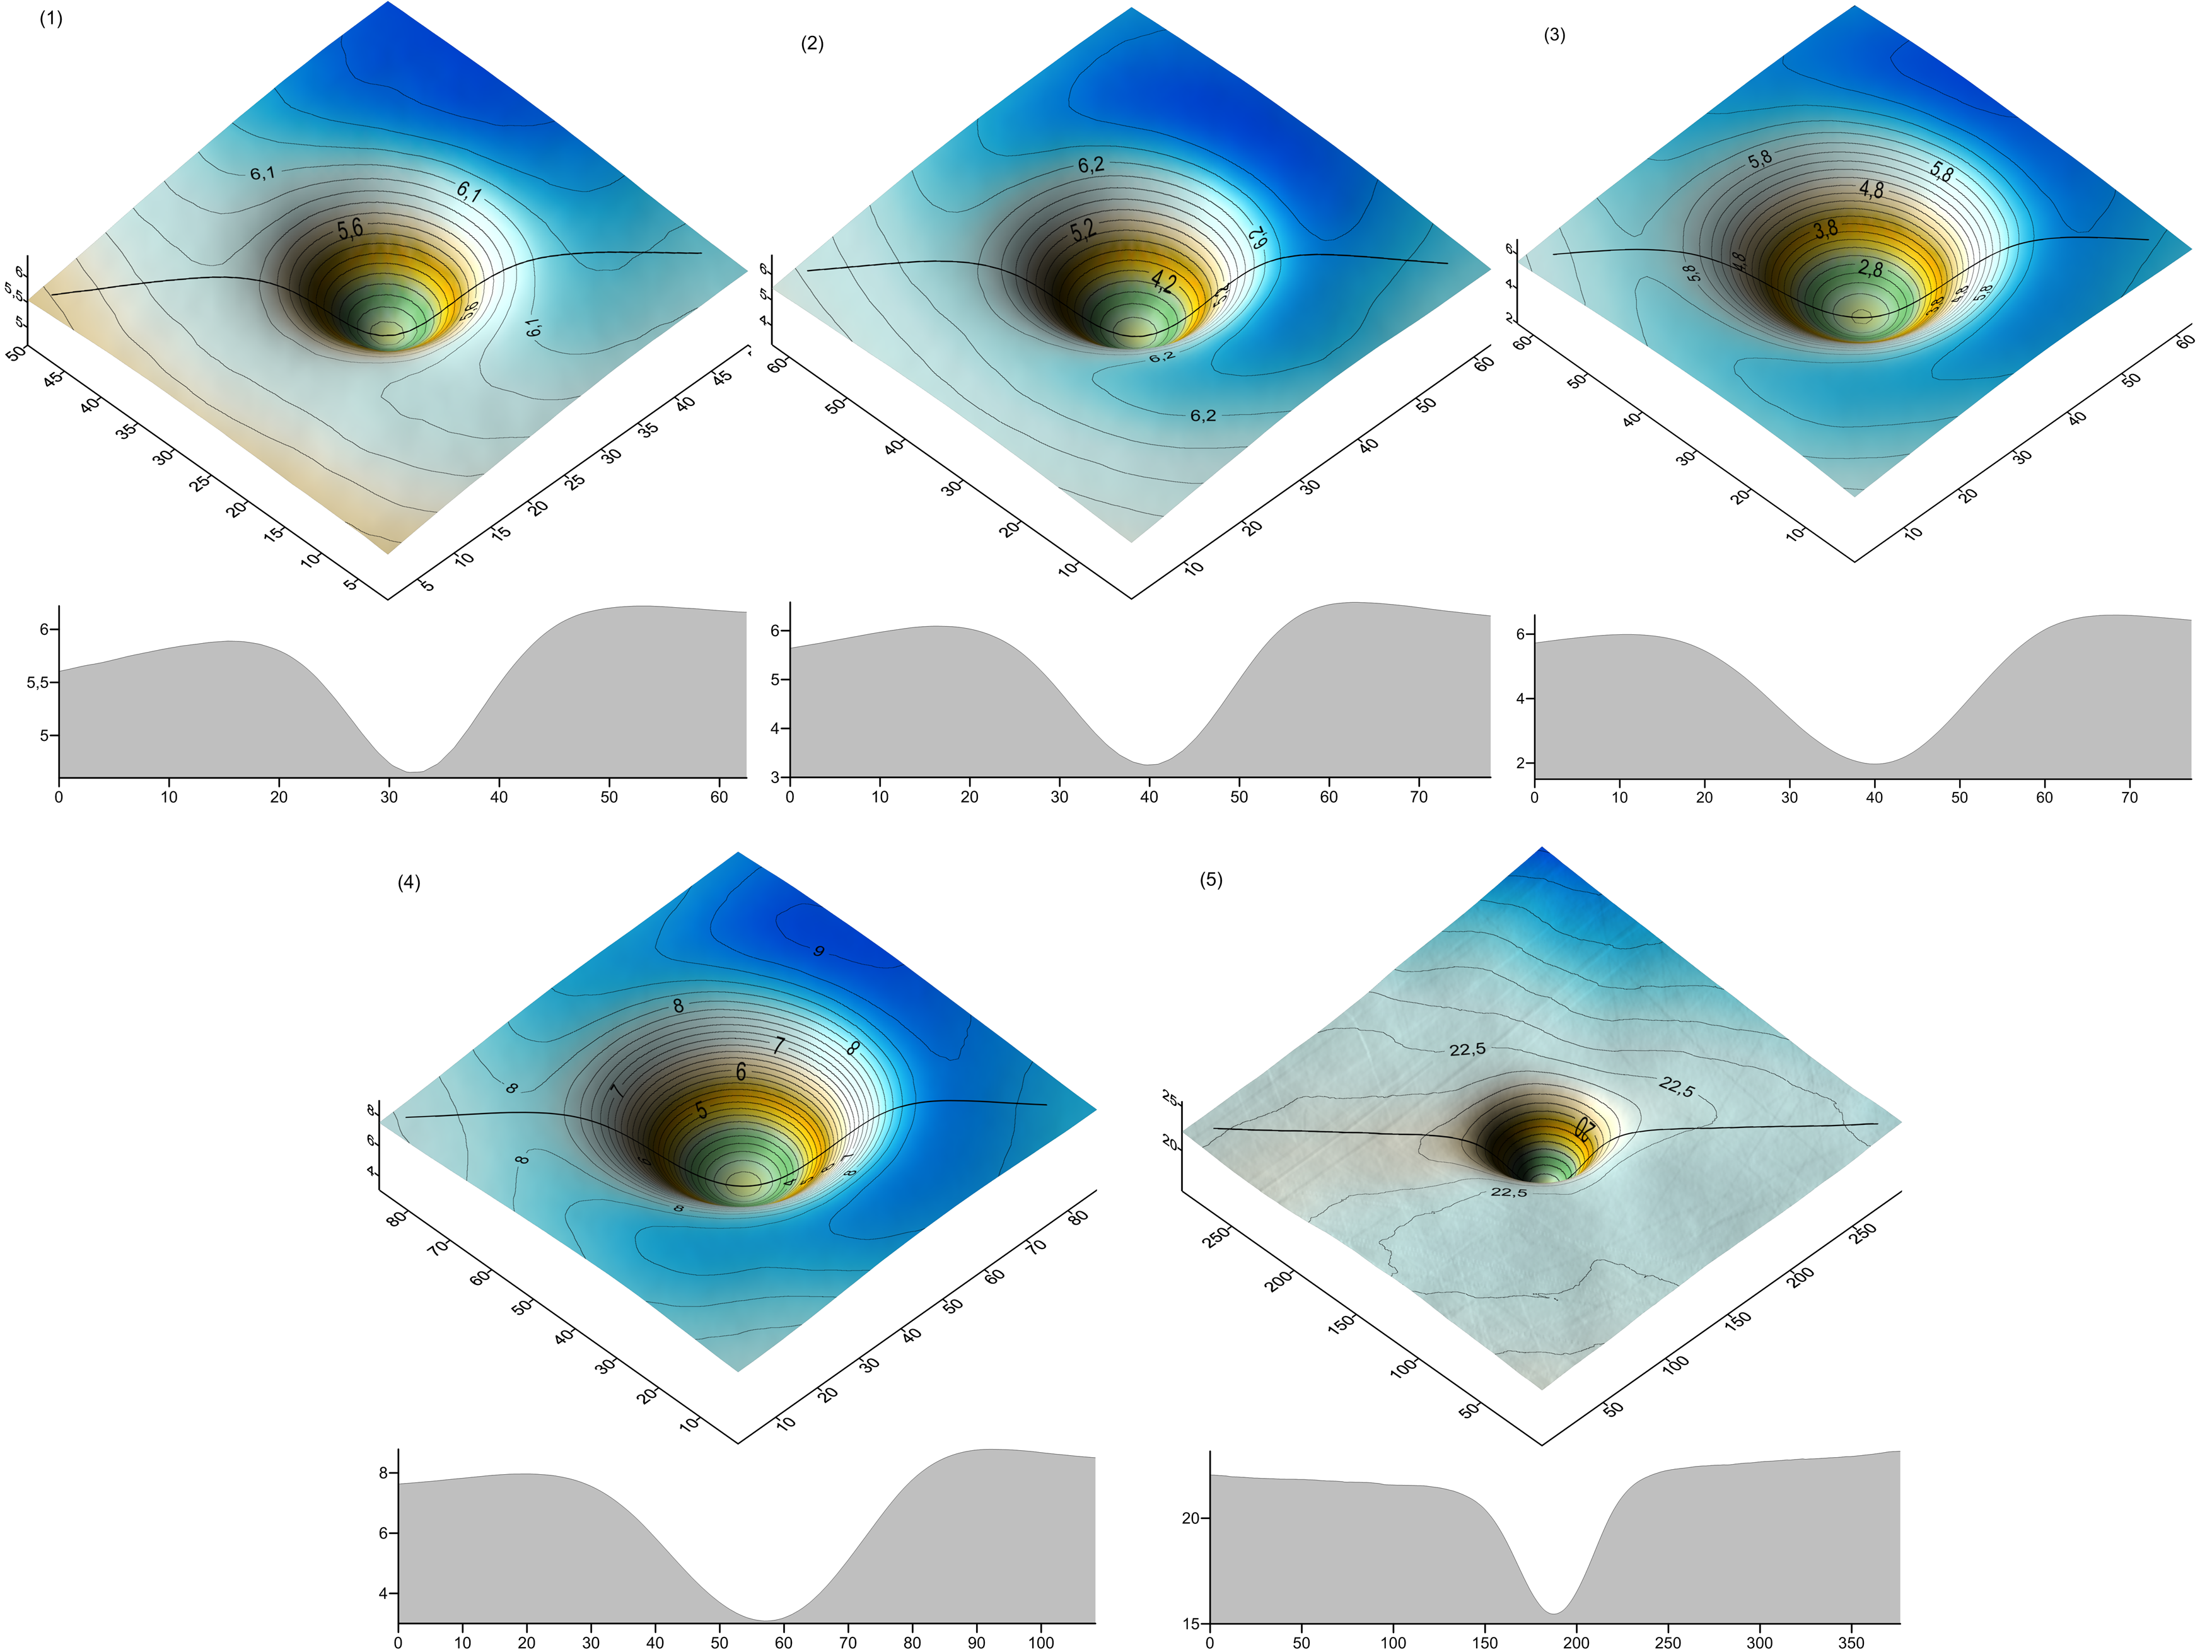
\includegraphics[width=19cm,angle=90]{slike/vrtace-po-razredih-menisija}
  \caption{Vrtače po velikosti razdelimo v pet razredov (najmanjša petina gre v prvi razred, itn.), in jih znotraj razredov povprečimo.}
  \label{fig:menisija-vrtace-po-razredih}
\end{figure}

Na prvi pogled se zdijo dobljeni profili gaussove oblike (\ref{fit-vrtace}), kar ne zbuja nujno zaupanja v metodo. Zdi pa se, da so oblike simetrične po kotu, torej lahko problem reduciramo na študij njihovih profilov. 

\begin{equation}
  f(x,y) = A \cdot e^{-\frac{(x-x_0)^2}{\sigma_x^2}-\frac{(y-y_0)^2}{\sigma_y^2}} + B \cdot x + C \cdot y + D  
  \label{fit-vrtace}
\end{equation}

Rezultat uporabimo tako da gaussovo funkcijo nalegamo na realne vrtače in tako dobimo dobre lokacije njihovih najnižjih točk, ter njihove $\sigma_x$ in $\sigma_y$. Z lokacijami najnižjih točk lahko izračunamo povprečne profile vrtač ($z(r)$), ki imajo enake efektivne polmere, naprimer: Slika \ref{fig:menisija-profil-21-fit}

\begin{figure}[H]
  \centering
  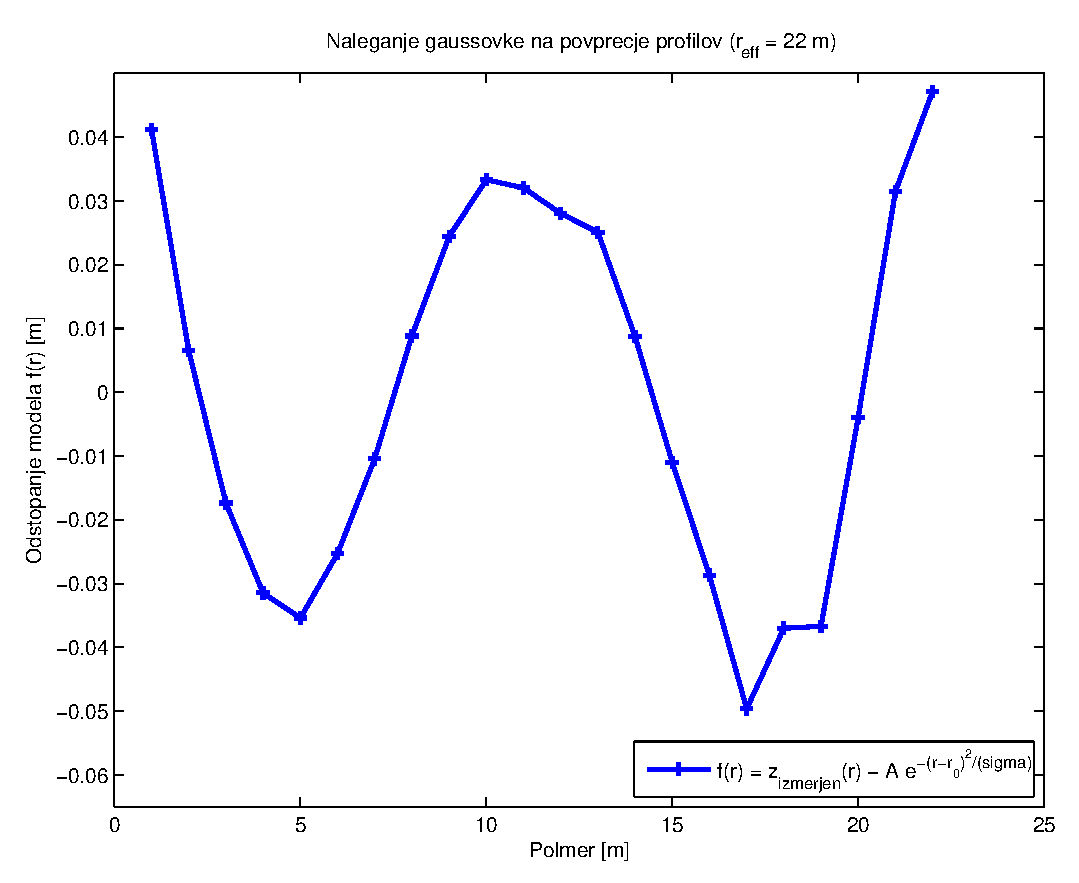
\includegraphics{slike/menisija-profil-21-fit}
  \caption{Povprecje profilov vrtač z efektivnimi polmeri med 21,5m in 22,5m. Prilegamo gaussovko (\ref{fit-profila}).}
  \label{fig:menisija-profil-21-fit}
\end{figure}

Če pa vse profile združimo v eno sliko, tako da polmer postavimo v smeri osi $y$ in efektivni polmer v smeri $x$ osi, dobimo sledečo sliko \ref{fig:menisija-profil-profilov}

\begin{figure}[H]
  \centering
  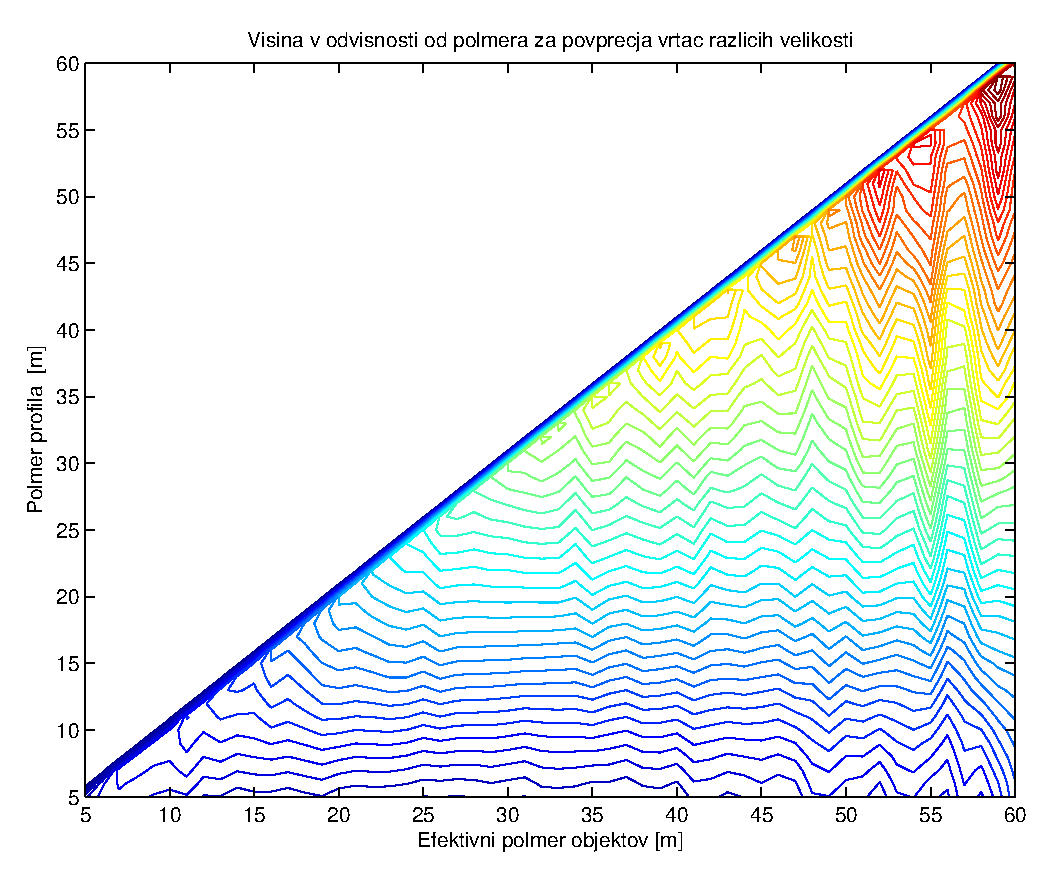
\includegraphics{slike/menisija-profil-profilov}
  \caption{Odvisnost profila vrtace od velikosti vrtace}
  \label{fig:menisija-profil-profilov}
\end{figure}

Zdi se torej, da so vrtače enake oblike ne glede na velikost in to po celi njihovi površini, le v okoliško površje se iztečejo prej ali kasneje, a zopet na podoben način.
Če na dobljene profile ponovno nalegamo gaussovko (\ref{fit-profila}) in izrišemo odvisnost $\sigma_x (r_{eff})$ vidimo, da to ne drži (Slika \ref{fig:menisija-sigma}).  
\begin{equation}
  f(r) = A \cdot e^{-\frac{(r-r_0)^2}{\sigma^2}} + C  
  \label{fit-profila}
\end{equation}

Odvisnost $\sigma_x(r_{eff})$ je iz naših podatkov težko določiti, zaenkrat poskusimo z eksponentno funkcijo (\ref{sigma-od-reff})


\begin{equation}
  \sigma (r_{eff}) = A \cdot e^{-\frac{r_{eff}-r_{eff_0}}{\sigma_{\sigma}}} + C 
  \label{sigma-od-reff}
\end{equation}

\begin{figure}[H]
  \centering
  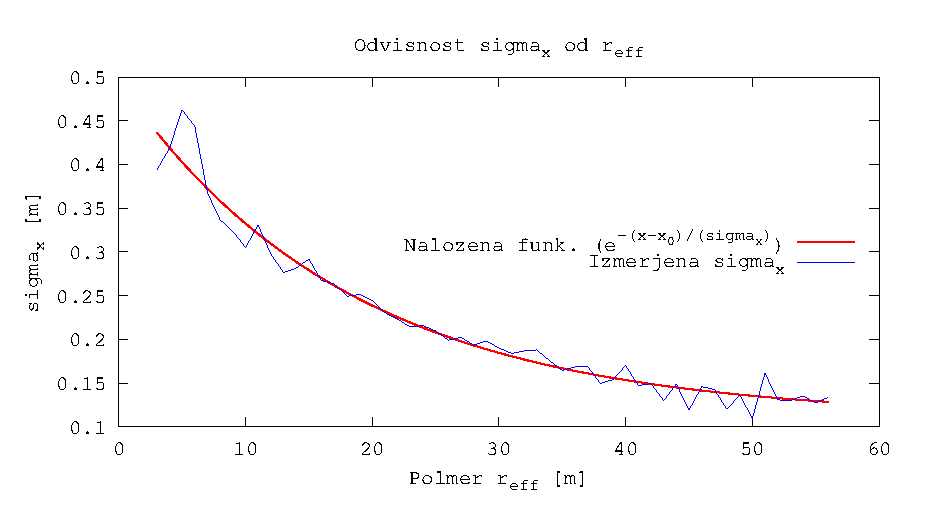
\includegraphics{slike/menisija-sigme}
  \caption{$\sigma$ s polmerom pada, torej večje kot so vrtače, bolj položna so njihova pobočja.}
  \label{fig:menisija-sigma}
\end{figure}

Na podlagi teh podatkov bi težko skleniti, da (\ref{fit-profila}) opiše profil idealne vrtače, a ujemanje je dobro in ga bomo uporabili za analitično modeliranje. 


\chapter{Analitično modeliranje vrtač}
\label{ch3}

\section{Difuzijski model}

Za izhodišče privzamemo difuzijski model, kot ga predlaga Heimsath \cite{Heimsath2001}.

\begin{figure}[H]
  \centering
  \begin{tikzpicture}[
    scale=1.8,
    arrow/.style={thick,->,shorten <=-2pt, shorten >=-2pt},
    media/.style={font={\footnotesize\sffamily}}
]

    \fill[color=black!5] (0,4) coordinate (a_1) -- (6,2.5) coordinate (a_2) -- (6,0.5) coordinate (b_2) -- (0,2) coordinate (b_1)-- cycle;
    \fill[color=black!10] (b_1) -- (b_2) -- (6,0.2) coordinate (c_2) -- (0,1.7) coordinate (c_1) -- cycle;
    \fill[color=black!25] (c_1) -- (c_2) -- (6,0) -- (0,0) -- cycle;

    \path[media] (1,2.8) node [rotate=-13.5] {Delno preperela}
                            (1,2.5) node [rotate=-13.5] {kamnina, $\rho_s$}
                            (2,0.6) node [rotate=-13.5] {Nepreperela kamnina, $\rho_r$}
                            (1.3,1.5) node [rotate=-13.5] {Preperevanje};

    % Draw surface, solid rock boundary and dz_b
    \draw [thick]               (a_1) -- (a_2) node [above, xshift=-5pt] {$z$};
    \draw [thick]               (b_1) -- (b_2) node [above, xshift=-5pt] {$z_b$};
    \draw [dashed,thick] (c_1) -- (c_2);

    % Draw dr volume
    \draw (2,1.5) -- (2,3.5);
    \draw (4,1) -- (4,3);

    %Draw currents
    \draw [arrow] (1.75,2.4375) -- (2.25,2.3125) node [above=1pt] {$q_s(r)$};
    \draw [arrow] (3.75,1.9375) -- (4.25,1.8125) node [above left =9pt] {$q_s(r+dr)$};
    \draw [arrow] (2.5,1.25) -- (2.5,1.55) node [above] {$\rho_r \frac{\partial z_b}{\partial t}$};
    \draw [arrow] (3.5,1.3) -- (3.5,0.6) node [above=36] {$Q_s$};
    \draw [arrow] (3,3.1) -- (3,3.45) node [below=18pt] {$\rho_s \frac{\partial h}{\partial t}$};

    % Draw h and dz_b
    \draw [<->] (5,0.75) -- (5,2.75) node [midway, right] {$h$};
    \draw [<->] (5,0.45) -- (5,0.75) node [midway, right, yshift=-0pt,rotate=-13.5] {$dz_b$};

    % Draw axes
    \draw [<->,thick] (0,4.3) node (yaxis) [above] {$z$}
        |- (6.3,0) node (xaxis) [right] {$r$};

\end{tikzpicture}
  \caption{Skica difuzijskega modela nastajanja vrtače}
  \label{fig:difuzijski-model}
\end{figure}

\begin{equation}
  \rho_s \frac{\partial h}{\partial t} = -\rho_r \frac{\partial z_b}{\partial t} - \nabla q_s
  \label{kontinuitetna-enacba-original}
\end{equation}

Kjer je $h$ višina stolpca sedimenta, $z_b$ višina skalne podlage, $z$ višina površja, $\rho_r$ in $\rho_s$ gostoti skalne podlage in sedimenta, $q_s$ pa gostota toka sedimenta. Za gostoto toka sedimenta vzamemo, da je sorazmeren z naklonom površja:
\begin{equation}
  q_s = - \rho_s K \nabla z
  \label{difuzijski-tok}
\end{equation}

Kjer je $K$ analogna konstanta difuzijski.
Model dopolnimo z raztapljanjem in izpiranjem delno raztopljene kamnine v podzemlje - to pospravimo v člen $Q_s$ in vstavimo \ref{difuzijski-tok}.
\begin{equation}
  \rho_s \frac{\partial h}{\partial t} = -\rho_r \frac{\partial z_b}{\partial t} + K \rho_s \Delta z - Q_s
  \label{kontinuitetna-enacba}
\end{equation}

Dobljen model skiciramo na Sliko \ref{fig:difuzijski-model}.

V ravnovesnem stanju vrtače, ki smo ga domnevno našli v \ref{realne-vrtace}. poglavju (enačba \ref{fit-profila}) zahtevamo, da velja $\frac{\partial h}{\partial t} = 0$ in $\frac{\partial z_b}{\partial t} = C$, kjer $C<0$, saj se meja preperelosti znižuje. Dobimo:

\begin{equation}
  Q_s = - \rho_r C + \rho_s K \Delta z
  \label{kontinuitetna-enacba-ravnovesje}
\end{equation}

Vstavimo ravnovesni profil vrtače (enačba \ref{fit-profila}) in vrednosti iz tabele (\ref{tab:tabela-konstant}), da dobimo profil $Q_s$ profil raztapljanja apnenca v na površju (Slika (\ref{fig:profil-raztapljanja})).

\begin{table}[h]
  \centering
  \begin{tabular}{| l | c | l | l |} \hline
    $\rho_r$ & $2700$ $kg/m^3$ & Gostota apnenca                                            \\ \hline
    $\rho_s$ & $1000$ $kg/m^3$ & Gostota delno preperele kamnine                            \\ \hline
    $C$      & $50 \cdot 10^{-6} m/leto$  & Hitrost preperevanja apnenca na ravnini         \\ \hline
    $K$      & $1 \cdot 10^{-4} m^2/leto$ & Difuzijska konstanta za delno preperelo kamnino \\ \hline
    $\sigma$ & $4.5m$ & $\sigma$ vrtače po nastavku (\ref{fit-profila})                     \\ \hline
    $A$      & $6m$ & Globina vrtače $A$ po nastavku (\ref{fit-profila})                    \\ \hline
  \end{tabular}
  \caption{Vrednosti iz literature \cite{Gams1967} \cite{ford2007karst} \cite{fleurant2008modelling} in \ref{realne-vrtace}. poglavja}
  \label{tab:tabela-konstant}
\end{table}

\begin{figure}[H]
  \begin{center}
    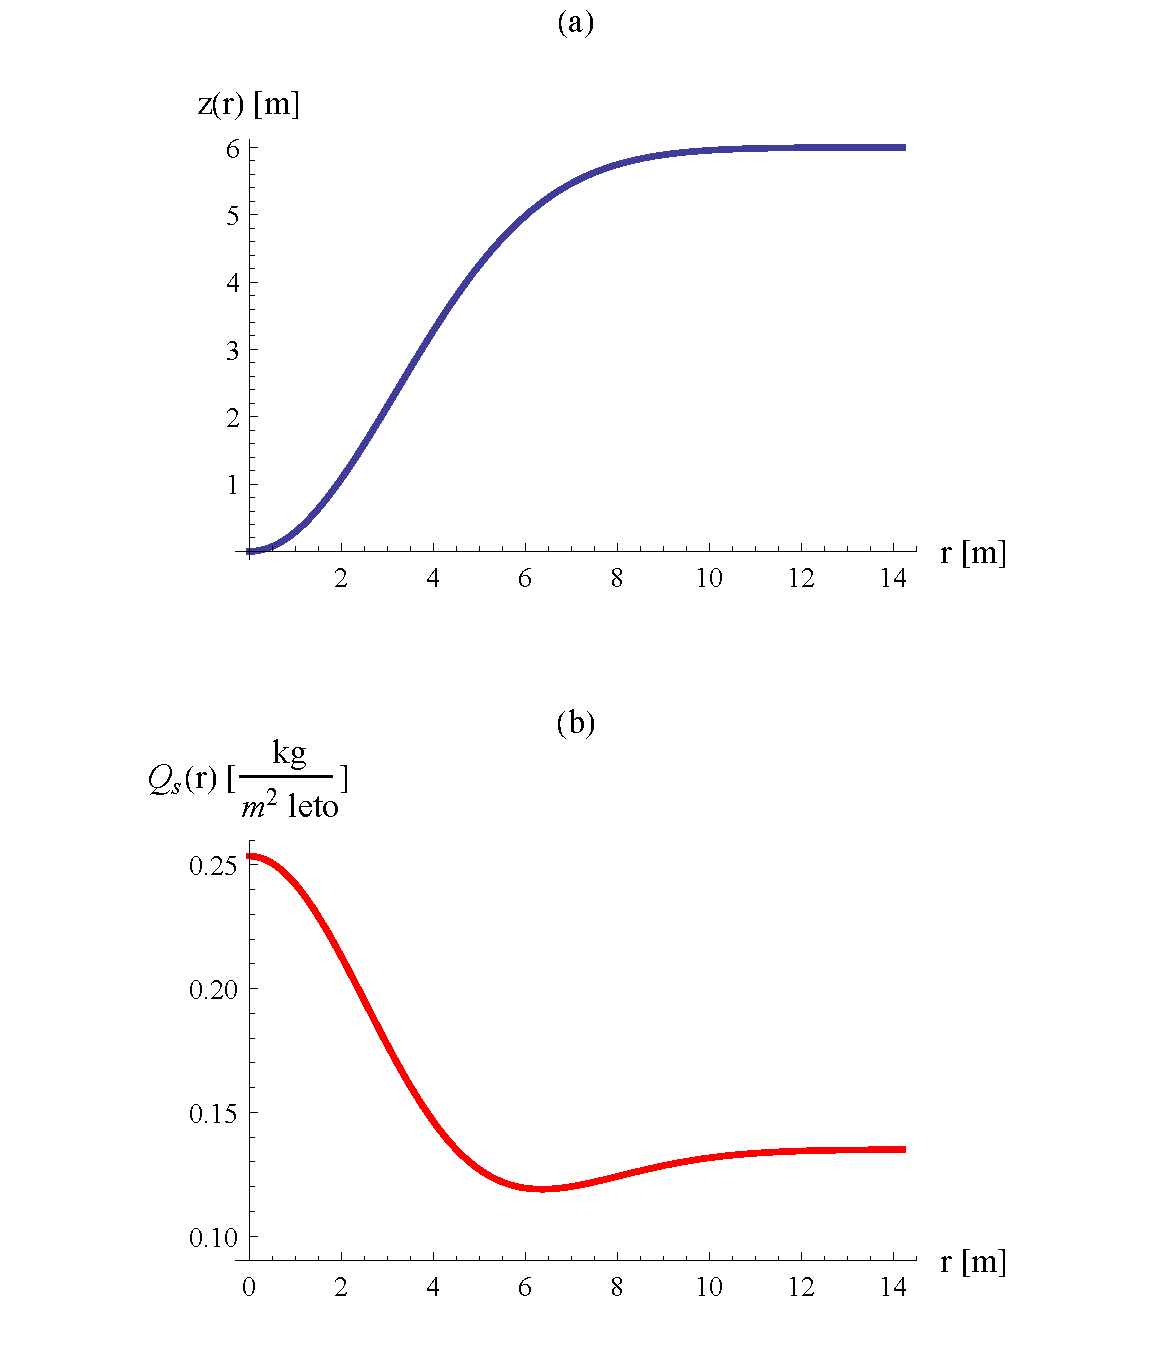
\includegraphics[width=10cm]{slike/profil-raztapljanja}
  \end{center}
  \caption{(a) Profil vrtače (b) modeliran profil raztapljanja delno preperele kamnine}
  \label{fig:profil-raztapljanja}
\end{figure}

Dobljeni profil raztapljanja nakazuje kvalitativno podobnost meritvam, ki jih je opravil Zambo (\cite{Zambo1997}) v osemdesetih (Slika \ref{fig:vrtaca-aggtelek}).

\begin{figure}[H]
  \begin{center}
    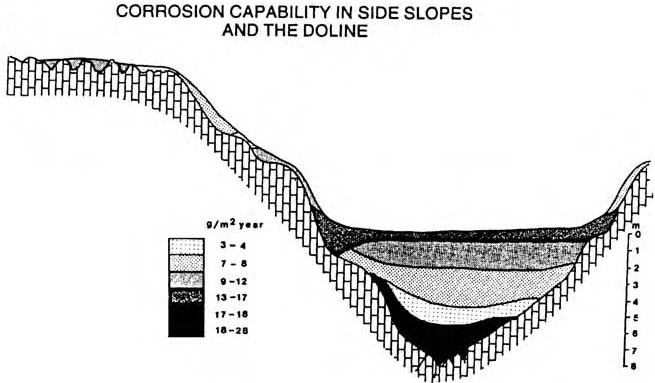
\includegraphics[width=10cm]{slike/vrtaca-aggtelek}
  \end{center}
  \caption{Meritve raztapljanja apnenca v realni vrtači - dolina Beke, nacionalni park Aggtelek na Madžarskem \cite{Zambo1997}}
  \label{fig:vrtaca-aggtelek}
\end{figure}

Profil vrtače blizu ravnovesja zmotimo s spremembo vrednosti oblike profila ($z(r)$), vstavimo nastavek za $\frac{\partial z_b}{\partial t}=\frac{1}{|h_0-h|}$ in \dots

\section{Elastomehanični model}
\section{Boussinesqov približek}


\chapter{Numerično modeliranje vrtač} 
\label{ch4}

\section{Model naključnih korozijskih točk}
\section{Naključne korozijske točke na realni kamnini}
\section{Preizkus modela korozijskih točk na geološki karti}

%%%%%%%%%%%%%%%%%%%%%%%%%%%%%%%%%%%%%%%%
\begin{comment}
%%%%%%%%%%%%%%%%%%%%%%%%%%%%%%%%%%%%%%%%

\chapter{Zaključek}


%%%%%%%%%%%%%%%%%%%%%%%%%%%%%%%%%%%%%%%%
\end{comment}
%%%%%%%%%%%%%%%%%%%%%%%%%%%%%%%%%%%%%%%%

\nocite{*}
\newpage
\bibliography{bibliography}{}
\bibliographystyle{alpha}


\end{document}

